% 
% Practica ICO
% ------------------
% Ingeniería del Conocimento
% Universidad de Granada
% 
% Autor:
% - María Carrasco Rodríguez
% 

\documentclass[a4paper,12pt,oneside]{book}
\usepackage[spanish]{babel}
\usepackage{graphicx}
\usepackage{ucs}
\usepackage{listings}
\usepackage[utf8]{inputenc}
\usepackage{amsfonts}
\usepackage{amssymb}
\usepackage{hyperref}
\usepackage{url}
\usepackage{multirow}
\usepackage{listings}  
\lstloadlanguages{Java}  
\lstset{language=Java,commentstyle=\emph}
\usepackage{color} 
\usepackage{colortbl}
\lstset{language=SQL}

\usepackage{phdthesis}



% opening
\title{Jugador Inteligente}
\author{María Carrasco Rodríguez \\
  Francisco Manuel Herrero Pérez}
\date{Curso 2009/10}
\parskip = 7 pt

\makeindex

\begin{document}
\begin{titlepage}
  \parskip = 6pt
  \null\vfil
  \hrule height 2pt
  \begin{center}
    \huge \textsf{\emph{ BattleTech}
      \\ \textbf{ Jugador Inteligente }}
    

    % \large \textit{\@subtitle}
  \end{center}
  \hrule height 2pt

  \begin{center}
    \large 
    María Carrasco Rodríguez \par 
    Francisco Manuel Herrero Pérez \par
    \vskip 15pt
    \hrule height 0.5pt
    \vskip 20pt
  \end{center}
  \begin{center}
    \small
    % \sffamily Universidad de Granada \par \vskip 1pt
    \sffamily Ingeniería del Conocimiento \par \vskip 1pt
    \footnotesize 
    \emph{Curso 09/10} \par
  \end{center}

  \vfil\null
\end{titlepage}


\tableofcontents

\pagebreak

\chapter{Introducción}
{\bf BattleTech} es un juego de combates entre enormes máquinas de
aspecto humanoide llamados {\it BattleMechs} (o más brevemente
llamados Mechs). \\


\chapter {Algoritmo A*}

El algoritmo de búsqueda A* es un tipo de algoritmo de búsqueda en
grafos. Se basa en encontrar, siempre y cuando se cumplan ciertas
condiciones, el camino de menor coste entre un nodo origen y uno
objetivo.\\

Nuestro objetivo es encontrar el camino más corto entre dos puntos
superando obstáculos (ya que en caso de que no hubiera obstáculos, es la
línea recta). Esta técnica muy usada en videojuegos de
estrategia y, en general en todos los videojuegos donde se trata la
inteligencia artificial. Por ello decidimos incorporarla a nuestra práctica.\\

La mayor ventaja de este algoritmo con respecto a otros es que tiene
en cuenta tanto el valor heurístico de los nodos como el coste real del
recorrido. Así, el algoritmo A* utiliza una función de evaluación:
$$f(n) = g(n) + h'(n) $$
Donde:
\begin {itemize}
\item {\bf h'(n)} Valor heurístico del nodo a evaluar desde el actual n
  hasta el final.
\item {\bf g(n)} Coste real del camino recorrido para llegar a dicho nodo, n.
\end {itemize}


A* mantiene dos estructuras de datos auxiliares:
\begin {itemize}
\item {\bf Abiertos}. Cola de prioridad, ordenada por el valor f(n) de
  cada nodo. (Lista de los nodos que necesitan ser comprobados)
\item {\bf Cerrados}. Guarda la información de los nodos que ya han
  sido visitados.
\end {itemize}
En cada paso del algoritmo se expande el nodo que esté primero en
abiertos, y en caso de que no sea un nodo objetivo, calcula la f(n) de
todos sus hijos, los inserta en abiertos, y pasa el nodo evaluado a cerrados.


\section {Implementación}

La implementación es genérica y no se basa en ningún juego en
concreto. {\bf PathFinder} es una clase genérica que no tiene en
cuenta como representes tu grafo ni como representes o como calcules
el coste de moverte de un lugar a otro. Deja a gusto del programador
especificar la información mediante el paso de funciones al constructor.

¿Cómo sabe {\it PathFinder} la forma de nuestro grafo? Sólo nos basta
con especificarlo en la función {\bf successors}. Esta función
especifica los sucesores de un node, que son aquellos nodos a los que
se puede llegar desde el nodo inicial en un solo paso. 

\begin{figure}[!h]
  \centering
  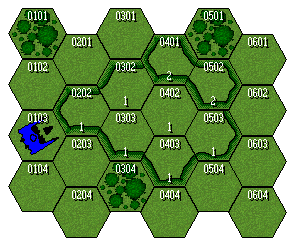
\includegraphics[width=7cm]{images/map2.png}
%  \caption{Trozo de mapa.}
\end{figure}

En nuestro ejemplo, los sucesores del nodo {\it 0103}, donde se encuentra
nuestro personaje, son: {\it 0102, 0202, 0203, 0104}


\newpage
\begin{thebibliography}{XXX}
\bibitem{0} González Duque, R., 2003. {\it PYTHON para todos.} $1^{st}$ed. \\
\bibitem{2} Gutschmidt, Tom, 2003. {\it Game Programming with Python,
    Lua, and Ruby  } Premier Press \\
\bibitem{3} Pilgrim, Mark, 2004. {\it Dive into Python.} Apress. \\
\bibitem{1}  \url{
    http://theory.stanford.edu/~amitp/GameProgramming/} \label{amit}
  \\
\bibitem{4}  \url{http://www.policyalmanac.org/games/aStarTutorial.htm}\\
\bibitem{5}  \url{ }\\
\bibitem{6}  \url{ }\\
\bibitem{7}  \url{ }
\end{thebibliography}

\end{document}
